\chapter{Classical Ciphers}

\begin{introduction}[Contents]
    \item Cipher
    \item Ceaser's Cipher
    \item Substitution Cipher
    \item One-time pad
\end{introduction}

\begin{figure}[h]
    \centering
    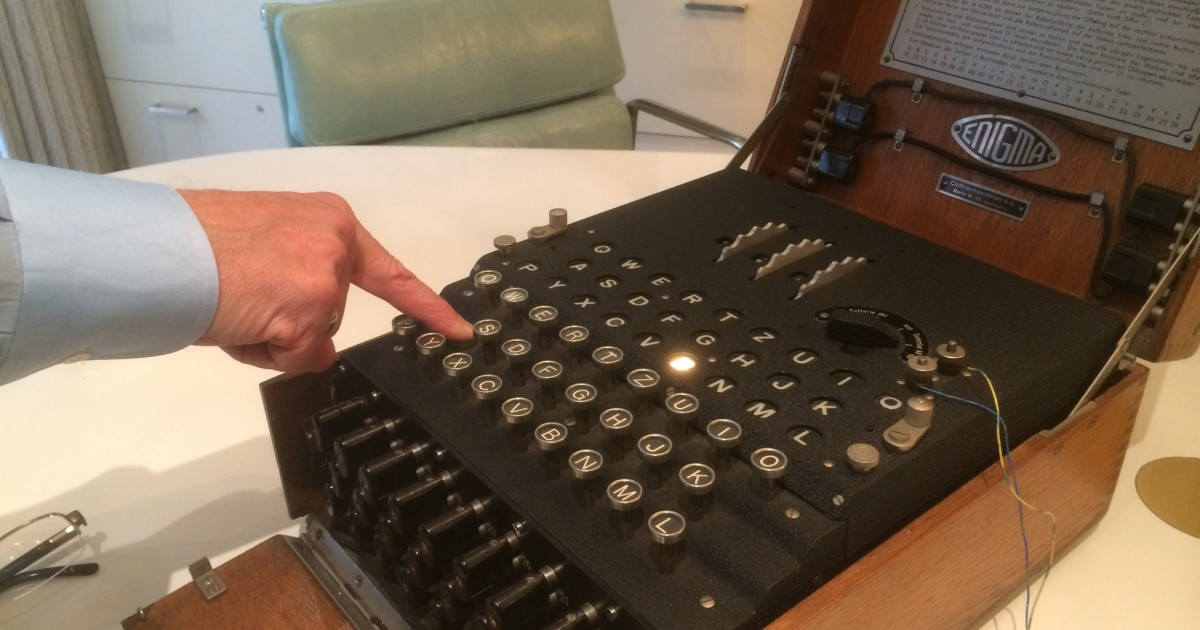
\includegraphics[width=0.5\textwidth]{enigma}
    \caption{The Enigma Machine used for encrypting messages during WWII}
\end{figure}

In this chapter, we will talk about ciphering techniques that are obsolete. However, a fair bit of history is interesting, as well as important.
We have made a tremendous progress in mathematics since the discovery of ciphers mentioned in this chapter. We have also achieved a gaint leap in our 
computing power. The way we communicate has changed drastically too, making the ideas mentioned in this chapter easily breakable. Let's learn it regardless.
\newpage

\section{Cipher}

\subsection{Definition}
\begin{definition}{Cipher}{}
Cipher is a collection of two functions -- the encryption function (\verb!E!), and the decryption function (\verb!D!).
\end{definition}
Let \verb!P!, \verb!C! be two sets where \verb!P! is a collection of all the plain texts, and \verb!C! is a collection of all the encrypted/cipher texts.
The encryption function \verb!E! maps all elements from \verb!P! $\rightarrow$ \verb!C! and the decryption function \verb!D! maps all elements from \verb!C!
$\rightarrow$ \verb!P!.

\subsection{Correction Criteria}
For any cipher to be correct, the following condition must satisfy: $\forall m \in P, D(E(m)) = m$. Meaning, the decryption of a encrypted message must give
back the original message, for all the original messages.

\newpage

\section{Ceaser Cipher}

This is one of the earliest known example of cryptgraphy and was used by Julius Ceaser. The cipher is very simple. To encrypt a message, you use the 
following replacement technique:
\begin{center}
    \emph{a $\rightarrow$ d, b $\rightarrow$ e, c $\rightarrow$ f, ..., x $\rightarrow$ a, y $\rightarrow$ b, z $\rightarrow$ c}
\end{center}

And to decrypt, you just replace it back, \emph{i.e.}:
\begin{center}
    \emph{d $\rightarrow$ a, e $\rightarrow$ b, c $\rightarrow$ f, ..., a $\rightarrow$ x, b $\rightarrow$ y, c $\rightarrow$ z}
\end{center}

\begin{example}
Encrypt \textbf{my name is james}, and decrypt it back.

To encrypt, you just replace each letter using the mapping. For instance, \textbf{m} is replaced with \textbf{p},
\textbf{y} is replaced with \textbf{b}, and so on to get \textbf{pb qdph lv mdphv}. Looks like giberish, Doesn't it?

Now to decrypt \textbf{pb qdph lv mdphv}, we just replace the word back or use the inverse mapping. For instance, \textbf{p} is replaced with \textbf{m},
\textbf{b} is replaced with \textbf{y}, and so on to get \textbf{my name is james}
\end{example}

To do more examples on your own, visit this link: \href{https://www.dcode.fr/caesar-cipher}{https://www.dcode.fr/caesar-cipher}
\newpage

\section{Substitution Cipher}
\lipsum
\newpage

\section{One-time pad}
\lipsum
\newpage


\begin{problemset}
    \item What type of function should be \verb!E! and \verb!D!? Surjective, Injective, Bijective?
    \item What if the correction criteria is not met?
\end{problemset}
\newpage